\section{A hajtáslánc modellezése}
\subsection{a) A motor és hajtómű azonosítása}
A paramétertáblázat alapján a rendszer névleges feszültsége $u_n = 30\text{ V}$, a hajtómű áttétele $N = 181:1$. Ennek megfelelően a MAXON katalógusokból a kiválasztott elemek:
\begin{itemize}
    \item \textbf{Motor:} MAXON A-MAX 26, 11 W (Cikkszám: 110943)
    \item \textbf{Hajtómű:} MAXON GP 26 A (Cikkszám: 406771)
\end{itemize}

A katalógusadatok alapján a rendszer paraméterei az alábbi táblázatban láthatók:

\begin{table}[H]
    \centering
    \begin{tabular}{|l|c|r|r|}
        \hline
        \textbf{Paraméter neve}  & \textbf{Jele} & \textbf{Katalógus adat} & \textbf{SI mértékegység}           \\ \hline
        Névleges feszültség      & $u_n$         & 30 V                    & 30 V                               \\ \hline
        Armatúra ellenállás      & $R$           & $19.1\ \Omega$          & $19.1\ \Omega$                     \\ \hline
        Armatúra induktivitás    & $L$           & 1.9 mH                  & $1.9 \cdot 10^{-3}$ H              \\ \hline
        Motorállandó             & $k_m$         & 40.1 mNm/A              & $40.1 \cdot 10^{-3}$ Nm/A          \\ \hline
        Forgórész tehetetlensége & $J_r$         & 12.6 $\text{gcm}^2$     & $1.26 \cdot 10^{-6}\ \text{kgm}^2$ \\ \hline
        Névleges áramerősség     & $i_n$         & 0.47 A                  & 0.47 A                             \\ \hline
        Áttétel                  & $N$           & 181 : 1                 & 181                                \\ \hline
        Viszkózus csillapítás    & $B$           & -                       & $2 \cdot 10^{-6}$ Nms/rad          \\ \hline
        Tárcsa tehetetlensége    & $J_t$         & 200 $\text{gcm}^2$      & $2 \cdot 10^{-5}\ \text{kgm}^2$    \\ \hline
    \end{tabular}
    \caption{A hajtáslánc azonosított paraméterei}
\end{table}

\newpage
\subsection{b) Struktúragráf}
A rendszer az alábbi egyenletekkel jellemezhető:
\begin{align}
    u(t) - R i(t) - L \frac{di(t)}{dt} - u_i(t)                        & = 0               \\
    u_i(t)                                                             & = k_m \omega_m(t) \\
    M_m(t)                                                             & = k_m i(t)        \\
    M_m(t) - J_r \frac{d\omega_m(t)}{dt} - B \omega_m(t) - M_{terh}(t) & = 0
\end{align}
Ebből a struktúragráf felépíthető az elektromos hálózat és a mechanikai oldal összekapcsolásával egy ideális váltó és hajtómű váltó segítségével.

\begin{figure}[H]
    \centering
    \resizebox{\linewidth}{!}{
        \begin{tikzpicture}[>=stealth, thick, font=\sffamily,
                midarrow/.style={decoration={markings, mark=at position 0.5 with {\arrow{>}}}, postaction={decorate}}]

            % Three ground lines (gaps centered under km and N circles)
            \draw[ultra thick] (0,0) -- (5.0,0);
            \node[below] at (2.5, 0) {$U_{\text{ref}}=0$};
            \draw[ultra thick] (5.6,0) -- (9.2,0);
            \node[below] at (7.4, 0) {$\omega_{\text{ref}}=0$};
            \draw[ultra thick] (9.8,0) -- (12.8,0);
            \node[below] at (11.3, 0) {$\omega_{\text{ref}}=0$};

            % U1, U2, U3 nodes
            \coordinate (U1) at (0.8, 1.8);
            \coordinate (U2) at (2.5, 3.2);
            \coordinate (U3) at (4.5, 1.8);

            % w1, w2 nodes
            \coordinate (w1) at (7.4, 2.3);
            \coordinate (w2) at (11.0, 2.8);

            % U_be source path
            \coordinate (UbeC) at (0.45, 0.8);
            \draw[thick] (0.3, 0) to[out=85, in=265] (UbeC) to[out=85, in=220] (U1);
            \draw[thick] (UbeC) circle (0.3);
            \draw[<-, thick] (0.05, 0.4) to[bend left=30] (0.05, 1.2);
            \node[left] at (0.0, 0.8) {$U_{be}$};

            \fill (U1) circle (2pt) node[above left] {$U_1$};

            % R arc
            \draw[thick, midarrow] (U1) to[out=50, in=170] node[above left] {$R$} (U2);
            \fill (U2) circle (2pt) node[below=0.1cm] {$U_2$};

            % L arc
            \draw[thick, midarrow] (U2) to[out=-10, in=130] node[above right] {$L$} (U3);
            \fill (U3) circle (2pt) node[below left] {$U_3$};

            % km transformer (single circle, center at 5.3, 0.8, radius 0.8)
            \coordinate (km) at (5.3, 0.8);
            \draw[thick] (km) circle (0.8);
            \node at (5.3, 1.85) {$k_m$};

            % U3 curves to upper-left of circle, w1 from upper-right
            \draw[thick] (U3) to[out=-60, in=135] (4.73, 1.37);
            \draw[thick] (5.87, 1.37) to[out=45, in=180] (w1);

            % Internal arrows: from entry points straight down to the ground line
            \draw[thick, ->] (4.73, 1.37) -- (4.73, 0);
            \draw[thick, ->] (5.87, 1.37) -- (5.87, 0);

            \fill (w1) circle (2pt) node[above] {$\omega_1$};

            % Jr and B (solid top with arrow, dashed below for Jr)
            \draw[thick, ->] (w1) to[out=-100, in=90] (7.0, 1.0);
            \draw[thick, dashed] (7.0, 1.0) -- (7.0, 0);
            \node[right] at (7.0, 0.5) {$J_r$};

            \draw[thick, ->] (w1) to[out=-60, in=90] (8.0, 0);
            \node[right] at (8.0, 0.8) {$B$};

            % N transformer (single circle, center at 9.5, 0.8, radius 0.8)
            \coordinate (N) at (9.5, 0.8);
            \draw[thick] (N) circle (0.8);
            \node at (9.5, 1.85) {$N$};

            % w1 curves to upper-left of circle, w2 from upper-right
            \draw[thick] (w1) to[out=-10, in=135] (8.93, 1.37);
            \draw[thick] (10.07, 1.37) to[out=45, in=150] (w2);

            % Internal arrows: from entry points straight down to the ground line
            \draw[thick, ->] (8.93, 1.37) -- (8.93, 0);
            \draw[thick, ->] (10.07, 1.37) -- (10.07, 0);

            \fill (w2) circle (2pt) node[above] {$\omega_2$};

            % Jt (solid top with arrow, dashed below for Jt)
            \draw[thick, ->] (w2) to[out=-80, in=90] (11.0, 1.2);
            \draw[thick, dashed] (11.0, 1.2) -- (11.0, 0);
            \node[left] at (11.0, 0.6) {$J_t$};

            % Mt source
            \coordinate (MtC) at (12.2, 0.8);
            \draw[thick] (w2) to[out=-20, in=90] (MtC) -- (12.2, 0);
            \fill[white] (MtC) circle (0.35);
            \draw[thick] (MtC) circle (0.35);
            \draw[thick] (11.9, 0.8) -- (12.5, 0.8);
            \draw[<-, thick] (12.7, 1.2) to[bend left=45] (12.7, 0.4);
            \node[right] at (12.8, 0.8) {$-M_t$};

        \end{tikzpicture}
    }
    \caption{A hajtáslánc struktúragráfja}
\end{figure}
\subsection{c) Impedanciahálózat}
Az elektromos és mechanikai oldal is impedanciákkal jellemezhető.
Az elektromos oldal impedanciája:
\begin{equation}
    Z_1(s) = R + s L
\end{equation}
A mechanikai forgórész impedanciája:
\begin{equation}
    Z_2(s) = \frac{1}{s J_r + B}
\end{equation}
A terhelés impedanciája a hajtómű után:
\begin{equation}
    Z_t(s) = \frac{1}{s J_t}
\end{equation}

\begin{figure}[H]
    \centering
    \resizebox{\linewidth}{!}{
        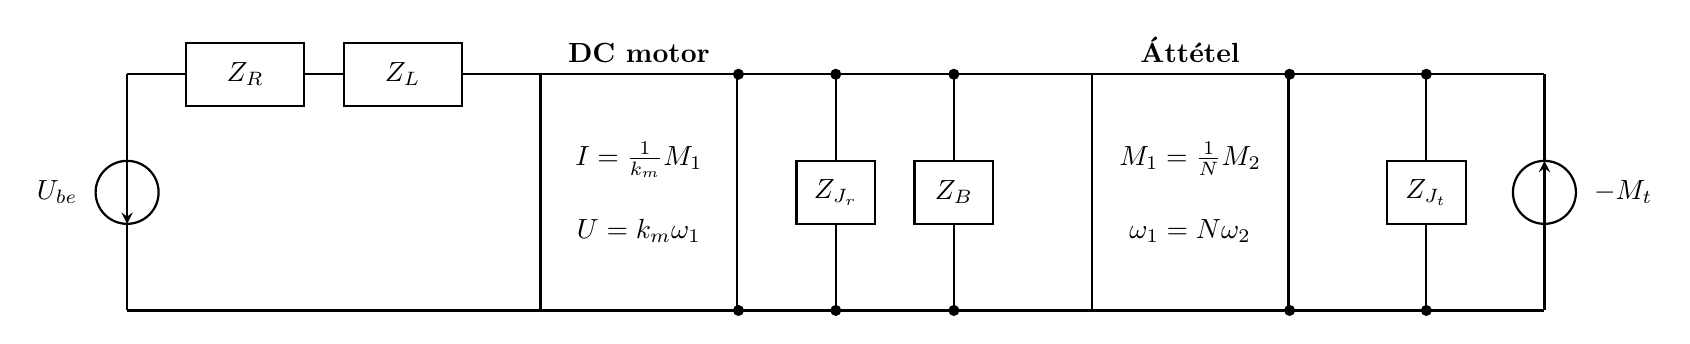
\begin{tikzpicture}[>=stealth, thick,
                block/.style={rectangle, draw, minimum width=1.5cm, minimum height=0.8cm, align=center},
                largeblock/.style={rectangle, draw, minimum width=2.5cm, minimum height=3cm, align=center}
            ]

            % Voltage source
            \draw[fill=white] (0,1.5) circle (0.4) node[left=0.5cm] {$U_{be}$};
            \draw[->] (0,1.9) -- (0,1.1);
            \draw (0,1.9) -- (0,3);
            \draw (0,1.1) -- (0,0);

            % ZR, ZL
            \node[block] (ZR) at (1.5, 3) {$Z_R$};
            \node[block] (ZL) at (3.5, 3) {$Z_L$};
            \draw (0,3) -- (ZR) -- (ZL);

            % Motor block
            \node[largeblock, label=above:{\textbf{DC motor}}] (motor) at (6.5, 1.5) {
                    $I = \frac{1}{k_m} M_1$\\[0.5cm]
                    $U = k_m \omega_1$
                };
            \draw (ZL) -- (motor.west |- 0,3);
            \draw (0,0) -- (motor.west |- 0,0);

            % Middle impedances ZJr, ZB
            \node[block, minimum width=1cm] (ZJr) at (9, 1.5) {$Z_{J_r}$};
            \node[block, minimum width=1cm] (ZB) at (10.5, 1.5) {$Z_B$};

            % Attétel block
            \node[largeblock, label=above:{\textbf{Áttétel}}] (att) at (13.5, 1.5) {
                    $M_1 = \frac{1}{N} M_2$\\[0.5cm]
                    $\omega_1 = N \omega_2$
                };

            \draw (motor.east |- 0,3) -- (att.west |- 0,3);
            \draw (motor.east |- 0,0) -- (att.west |- 0,0);

            \draw (9, 3) -- (ZJr.north); \draw (ZJr.south) -- (9, 0);
            \draw (10.5, 3) -- (ZB.north); \draw (ZB.south) -- (10.5, 0);
            \fill (9, 3) circle (2pt); \fill (9, 0) circle (2pt);
            \fill (10.5, 3) circle (2pt); \fill (10.5, 0) circle (2pt);
            \fill (motor.east |- 0,3) circle (2pt); \fill (motor.east |- 0,0) circle (2pt);

            % Right side
            \node[block, minimum width=1cm] (ZJt) at (16.5, 1.5) {$Z_{J_t}$};
            \draw (att.east |- 0,3) -- (18, 3);
            \draw (att.east |- 0,0) -- (18, 0);
            \fill (att.east |- 0,3) circle (2pt); \fill (att.east |- 0,0) circle (2pt);

            \draw (16.5, 3) -- (ZJt.north); \draw (ZJt.south) -- (16.5, 0);
            \fill (16.5, 3) circle (2pt); \fill (16.5, 0) circle (2pt);

            % Mt Effort Source
            \draw[fill=white] (18,1.5) circle (0.4) node[right=0.5cm] {$-M_t$};
            \draw[<-] (18,1.9) -- (18,1.1);
            \draw (18,1.9) -- (18,3);
            \draw (18,1.1) -- (18,0);

        \end{tikzpicture}
    }
    \caption{A rendszer impedanciahálózata}
\end{figure}

\subsection{d) Négypólusok kiküszöbölése}
Redukálom a teljes hálózatot a hajtómű kihajtó oldalára (tárcsa oldala).
Az elektromos impedancia redukálva:
\begin{equation}
    Z_{12}(s) = \frac{Z_1(s)}{k_m^2 N^2} = \frac{R + s L}{k_m^2 N^2}
\end{equation}
A motor belső mechanikai impedanciája redukálva:
\begin{equation}
    Z_{22}(s) = \frac{Z_2(s)}{N^2} = \frac{1}{N^2 (s J_r + B)}
\end{equation}
Az eredő "belső" impedancia, ami a motor és áttétel együtteséből adódik:
\begin{equation}
    Z_e(s) = \frac{Z_{22}(s) Z_t(s)}{Z_{22}(s) + Z_t(s)}
\end{equation}

\begin{figure}[H]
    \centering
    \resizebox{\linewidth}{!}{
        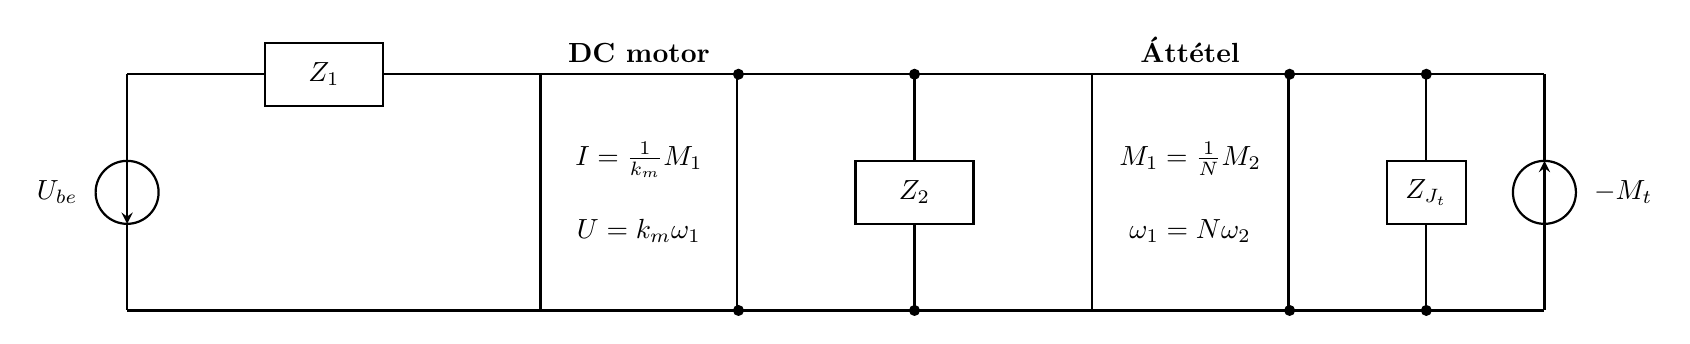
\begin{tikzpicture}[>=stealth, thick,
                block/.style={rectangle, draw, minimum width=1.5cm, minimum height=0.8cm, align=center},
                largeblock/.style={rectangle, draw, minimum width=2.5cm, minimum height=3cm, align=center}
            ]

            % Voltage source
            \draw[fill=white] (0,1.5) circle (0.4) node[left=0.5cm] {$U_{be}$};
            \draw[->] (0,1.9) -- (0,1.1);
            \draw (0,1.9) -- (0,3);
            \draw (0,1.1) -- (0,0);

            % Z1
            \node[block] (Z1) at (2.5, 3) {$Z_1$};
            \draw (0,3) -- (Z1);

            % Motor block
            \node[largeblock, label=above:{\textbf{DC motor}}] (motor) at (6.5, 1.5) {
                    $I = \frac{1}{k_m} M_1$\\[0.5cm]
                    $U = k_m \omega_1$
                };
            \draw (Z1) -- (motor.west |- 0,3);
            \draw (0,0) -- (motor.west |- 0,0);

            % Middle impedance Z2
            \node[block, minimum width=1.5cm] (Z2) at (10, 1.5) {$Z_2$};

            % Attétel block
            \node[largeblock, label=above:{\textbf{Áttétel}}] (att) at (13.5, 1.5) {
                    $M_1 = \frac{1}{N} M_2$\\[0.5cm]
                    $\omega_1 = N \omega_2$
                };

            \draw (motor.east |- 0,3) -- (att.west |- 0,3);
            \draw (motor.east |- 0,0) -- (att.west |- 0,0);

            \draw (10, 3) -- (Z2.north); \draw (Z2.south) -- (10, 0);
            \fill (10, 3) circle (2pt); \fill (10, 0) circle (2pt);
            \fill (motor.east |- 0,3) circle (2pt); \fill (motor.east |- 0,0) circle (2pt);

            % Right side
            \node[block, minimum width=1cm] (ZJt) at (16.5, 1.5) {$Z_{J_t}$};
            \draw (att.east |- 0,3) -- (18, 3);
            \draw (att.east |- 0,0) -- (18, 0);
            \fill (att.east |- 0,3) circle (2pt); \fill (att.east |- 0,0) circle (2pt);

            \draw (16.5, 3) -- (ZJt.north); \draw (ZJt.south) -- (16.5, 0);
            \fill (16.5, 3) circle (2pt); \fill (16.5, 0) circle (2pt);

            % Mt Effort Source
            \draw[fill=white] (18,1.5) circle (0.4) node[right=0.5cm] {$-M_t$};
            \draw[<-] (18,1.9) -- (18,1.1);
            \draw (18,1.9) -- (18,3);
            \draw (18,1.1) -- (18,0);

        \end{tikzpicture}
    }
    \caption{Az egyesített teljes impedanciahálózat}
\end{figure}

\subsection{e) Kapocsfeszültség és tárcsa szögsebesség átviteli függvény}
Az eredő rendszerben az átviteli függvény felírható:
\begin{equation}
    W_1(s) = \frac{\Omega_t(s)}{U(s)} = \frac{Z_e(s)}{(Z_{12}(s) + Z_e(s)) k_m N}
\end{equation}
Behelyettesítve az értékeket a kiszámított kifejezés így alakul:
\begin{equation}
    W_1(s) = \frac{7.2581}{7.847 \cdot 10^{-5} s^{2} + 0.7889 s + 53.9315}
\end{equation}

\newpage
\subsection{f) Átmeneti függvény ábrázolása}
A rendszer step (ugrás) válasza $W_1(s)$ alapján:
\begin{figure}[H]
    \centering
    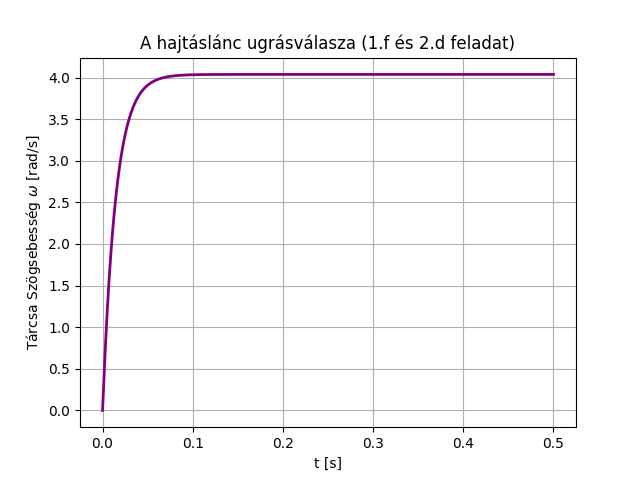
\includegraphics[width=0.8\textwidth]{res/imgs/fig_HajtaslancUgras.png}
    \caption{A $W_1(s)$ átviteli függvény ugrásválasza névleges feszültség mellett}
\end{figure}

\subsection{g) A modell időállandói}
Az átviteli függvény nevezőjének gyökei határozzák meg a rendszer időállandóit ($T_i = -1/p_i$).
\begin{equation}
    T_1 \approx 0.01453 \text{ s} \quad \text{és} \quad T_2 \approx 0.000100 \text{ s}
\end{equation}
